
%%%%%%%%%%%%%%%%%%%%%%%%%%%%%%%%%%%%%%%%%%%%%%%%%%%%%%
%   TeXstudio as your IDE
%%  برای compile در TeXstudio تنها کافی است منوی Options->Configure TeXstudio را زده و در پنجره Configure TeXstudio در بخش Build گزینه Default Compiler را به XeLaTeX تغییر دهید. سند شما به راحتی compile خواهد شد.
%   F1 & F5 : Build & view
%   F6      : Compile
%   F7      : View
%   --------------
%%%%%%%%%%%%%%%%%%%%%%%%%%%%%%%%%%%%%%%%%%%%%%%%%%%%%%
%%%% !TEX TS-program = XeLaTeX

\documentclass[oneside,bsc,12pt]{AUTthesis}

%       و دیگر بسته‌ها و ... در این فایل قرار دارد و بهتر است که با نحوه استفاده از آنها آشنا شوید. توجه شود برای نسخه نهایی پایان‌نامه حتماً hyperref را 
%        غیرفعال کنید.
\usepackage[ruled,vlined]{algorithm2e}

% در این فایل، دستورها و تنظیمات مورد نیاز، آورده شده است.
%-------------------------------------------------------------------------------------------------------------------
% در ورژن جدید زی‌پرشین برای تایپ متن‌های ریاضی، این سه بسته، حتماً باید فراخوانی شود.
\usepackage{amsthm,amssymb,amsmath,amsfonts}
% بسته‌ای برای تنطیم حاشیه‌های بالا، پایین، چپ و راست صفحه
\usepackage[top=30mm, bottom=30mm, left=25mm, right=30mm]{geometry}
% بسته‌‌ای برای ظاهر شدن شکل‌ها و تصاویر متن
\usepackage{graphicx}
\usepackage{color}
%بسته‌ای برای تنظیم فاصله عمودی خط‌های متن
\usepackage{setspace}
\usepackage{titletoc}
\usepackage{tocloft}
%با فعال کردن بسته زیر فوت‌نوت‌ها در هر صفحه ریست می‌شوند. حالت پیش‌فرض آن ریست شدن در هر فصل می‌باشد.
%\usepackage[perpage]{footmisc}
\usepackage{enumitem}
%\usepackage{titlesec}
% بسته‌ و دستوراتی برای ایجاد لینک‌های رنگی با امکان جهش
\usepackage[pagebackref=false,colorlinks,linkcolor=blue,citecolor=red]{hyperref}
\usepackage[nameinlink]{cleveref}%capitalize,,noabbrev
 \AtBeginDocument{%
    \crefname{equation}{برابری}{equations}%
    \crefname{chapter}{فصل}{chapters}%
    \crefname{section}{بخش}{sections}%
    \crefname{appendix}{پیوست}{appendices}%
    \crefname{enumi}{مورد}{items}%
    \crefname{footnote}{زیرنویس}{footnotes}%
    \crefname{figure}{شکل}{figures}%
    \crefname{table}{جدول}{tables}%
    \crefname{theorem}{قضیه}{theorems}%
    \crefname{lemma}{لم}{lemmas}%
    \crefname{corollary}{نتیجه}{corollaries}%
    \crefname{proposition}{گزاره}{propositions}%
    \crefname{definition}{تعریف}{definitions}%
    \crefname{result}{نتیجه}{results}%
    \crefname{example}{مثال}{examples}%
    \crefname{remark}{نکته}{remarks}%
    \crefname{note}{یادداشت}{notes}%
}
% چنانچه قصد پرینت گرفتن نوشته خود را دارید، خط بالا را غیرفعال و  از دستور زیر استفاده کنید چون در صورت استفاده از دستور زیر‌‌، 
% لینک‌ها به رنگ سیاه ظاهر خواهند شد که برای پرینت گرفتن، مناسب‌تر است
%\usepackage[pagebackref=false]{hyperref}
% بسته‌ لازم برای تنظیم سربرگ‌ها
\usepackage{fancyhdr}
% بسته‌ای برای ظاهر شدن «مراجع»  در فهرست مطالب
\usepackage[nottoc]{tocbibind}
% دستورات مربوط به ایجاد نمایه
\usepackage{makeidx,multicol}
\setlength{\columnsep}{1.5cm}

%%%%%%%%%%%%%%%%%%%%%%%%%%
\usepackage{verbatim}
\makeindex
\usepackage{sectsty}
% فراخوانی بسته زی‌پرشین و تعریف قلم فارسی و انگلیسی
\usepackage{xepersian}%[extrafootnotefeatures]
\SepMark{-}
%حتماً از تک لایو 2014 استفاده کنید.
\settextfont[Scale=1.2]{B Nazanin}
\setlatintextfont{Times New Roman}
\renewcommand{\labelitemi}{$\bullet$}
%%%%%%%%%%%%%%%%%%%%%%%%%%
% چنانچه می‌خواهید اعداد در فرمول‌ها، انگلیسی باشد، خط زیر را غیرفعال کنید.
%در غیر اینصورت حتماً فونت PGaramond را نصب کنید.
%\setdigitfont[Scale=1.1]{Yas}%%Yas
%%%%%%%%%%%%%%%%%%%%%%%%%%
% تعریف قلم‌های فارسی اضافی برای استفاده در بعضی از قسمت‌های متن
\defpersianfont\nastaliq[Scale=2]{IranNastaliq}
\defpersianfont\chapternumber[Scale=3]{B Nazanin}
%\chapterfont{\centering}%
%%%%%%%%%%%%%%%%%%%%%%%%%%
% دستوری برای تغییر نام کلمه «اثبات» به «برهان»
\renewcommand\proofname{\textbf{برهان}}

% دستوری برای تغییر نام کلمه «کتاب‌نامه» به «منابع و مراجع«
\renewcommand{\bibname}{منابع و مراجع}


% Headings for every page of ToC, LoF and Lot
\setlength{\cftbeforetoctitleskip}{-1.2em}
\setlength{\cftbeforelottitleskip}{-1.2em}
\setlength{\cftbeforeloftitleskip}{-1.2em}
\setlength{\cftaftertoctitleskip}{-1em}
\setlength{\cftafterlottitleskip}{-1em}
\setlength{\cftafterloftitleskip}{-1em}
%%\makeatletter
%%%%\renewcommand{\l@chapter}{\@dottedtocline{1}{1em\bfseries}{1em}}
%%%%\renewcommand{\l@section}{\@dottedtocline{2}{2em}{2em}}
%%%%\renewcommand{\l@subsection}{\@dottedtocline{3}{3em}{3em}}
%%%%\renewcommand{\l@subsubsection}{\@dottedtocline{4}{4em}{4em}}
%%%%\makeatother


\newcommand\tocheading{\par عنوان\hfill صفحه \par}
\newcommand\lofheading{\hspace*{.5cm}\figurename\hfill صفحه \par}
\newcommand\lotheading{\hspace*{.5cm}\tablename\hfill صفحه \par}

\renewcommand{\cftchapleader}{\cftdotfill{\cftdotsep}}
\renewcommand{\cfttoctitlefont}{\hspace*{\fill}\LARGE\bfseries}%\Large
\renewcommand{\cftaftertoctitle}{\hspace*{\fill}}
\renewcommand{\cftlottitlefont}{\hspace*{\fill}\LARGE\bfseries}%\Large
\renewcommand{\cftafterlottitle}{\hspace*{\fill}}
\renewcommand{\cftloftitlefont}{\hspace*{\fill}\LARGE\bfseries}
\renewcommand{\cftafterloftitle}{\hspace*{\fill}}

%%%%%%%%%%%%%%%%%%%%%%%%%%
% تعریف و نحوه ظاهر شدن عنوان قضیه‌ها، تعریف‌ها، مثال‌ها و ...
%برای شماره گذاری سه تایی قضیه ها
\theoremstyle{definition}
\newtheorem{definition}{تعریف}[section]
\newtheorem{remark}[definition]{نکته}
\newtheorem{note}[definition]{یادداشت}
\newtheorem{example}[definition]{نمونه}
\newtheorem{question}[definition]{سوال}
\newtheorem{remember}[definition]{یاداوری}
\theoremstyle{theorem}
\newtheorem{theorem}[definition]{قضیه}
\newtheorem{lemma}[definition]{لم}
\newtheorem{proposition}[definition]{گزاره}
\newtheorem{corollary}[definition]{نتیجه}
%%%%%%%%%%%%%%%%%%%%%%%%
%%%%%%%%%%%%%%%%%%%
%%% برای شماره گذاری چهارتایی قضیه ها و ...
%%\newtheorem{definition1}[subsubsection]{تعریف}
%%\newtheorem{theorem1}[subsubsection]{قضیه}
%%\newtheorem{lemma1}[subsubsection]{لم}
%%\newtheorem{proposition1}[subsubsection]{گزاره}
%%\newtheorem{corollary1}[subsubsection]{نتیجه}
%%\newtheorem{remark1}[subsubsection]{نکته}
%%\newtheorem{example1}[subsubsection]{مثال}
%%\newtheorem{question1}[subsubsection]{سوال}

%%%%%%%%%%%%%%%%%%%%%%%%%%%%

% دستورهایی برای سفارشی کردن صفحات اول فصل‌ها
\makeatletter
\newcommand\mycustomraggedright{%
 \if@RTL\raggedleft%
 \else\raggedright%
 \fi}
\def\@makechapterhead#1{%
\thispagestyle{style1}
\vspace*{20\p@}%
{\parindent \z@ \mycustomraggedright
\ifnum \c@secnumdepth >\m@ne
\if@mainmatter

\bfseries{\Huge \@chapapp}\small\space {\chapternumber\thechapter}
\par\nobreak
\vskip 0\p@
\fi
\fi
\interlinepenalty\@M 
\Huge \bfseries #1\par\nobreak
\vskip 120\p@

}

%\thispagestyle{empty}
\newpage}
\bidi@patchcmd{\@makechapterhead}{\thechapter}{\tartibi{chapter}}{}{}
\bidi@patchcmd{\chaptermark}{\thechapter}{\tartibi{chapter}}{}{}
\makeatother

\pagestyle{fancy}
\renewcommand{\chaptermark}[1]{\markboth{\chaptername~\tartibi{chapter}: #1}{}}

\fancypagestyle{style1}{
\fancyhf{} 
\fancyfoot[c]{\thepage}
\fancyhead[R]{\leftmark}%
\renewcommand{\headrulewidth}{1.2pt}
}


\fancypagestyle{style2}{
\fancyhf{}
\fancyhead[R]{چکیده}
\fancyfoot[C]{\thepage{}}
\renewcommand{\headrulewidth}{1.2pt}
}

\fancypagestyle{style3}{%
  \fancyhf{}%
  \fancyhead[R]{فهرست نمادها}
  \fancyfoot[C]{\thepage}%
  \renewcommand{\headrulewidth}{1.2pt}%
}

\fancypagestyle{style4}{%
  \fancyhf{}%
  \fancyhead[R]{فهرست جداول}
  \fancyfoot[C]{\thepage}%
  \renewcommand{\headrulewidth}{1.2pt}%
}

\fancypagestyle{style5}{%
  \fancyhf{}%
  \fancyhead[R]{فهرست اشکال}
  \fancyfoot[C]{\thepage}%
  \renewcommand{\headrulewidth}{1.2pt}%
}

\fancypagestyle{style6}{%
  \fancyhf{}%
  \fancyhead[R]{فهرست مطالب}
  \fancyfoot[C]{\thepage}%
  \renewcommand{\headrulewidth}{1.2pt}%
}

\fancypagestyle{style7}{%
  \fancyhf{}%
  \fancyhead[R]{نمایه}
  \fancyfoot[C]{\thepage}%
  \renewcommand{\headrulewidth}{1.2pt}%
}

\fancypagestyle{style8}{%
  \fancyhf{}%
  \fancyhead[R]{منابع و مراجع}
  \fancyfoot[C]{\thepage}%
  \renewcommand{\headrulewidth}{1.2pt}%
}
\fancypagestyle{style9}{%
  \fancyhf{}%
  \fancyhead[R]{واژه‌نامه‌ی فارسی به انگلیسی}
  \fancyfoot[C]{\thepage}%
  \renewcommand{\headrulewidth}{1.2pt}%
}
%


%دستور حذف نام لیست تصاویر و لیست جداول از فهرست مطالب
\newcommand*{\BeginNoToc}{%
  \addtocontents{toc}{%
    \edef\protect\SavedTocDepth{\protect\the\protect\value{tocdepth}}%
  }%
  \addtocontents{toc}{%
    \protect\setcounter{tocdepth}{-10}%
  }%
}
\newcommand*{\EndNoToc}{%
  \addtocontents{toc}{%
    \protect\setcounter{tocdepth}{\protect\SavedTocDepth}%
  }%
}
\newcounter{savepage}
\renewcommand{\listfigurename}{فهرست اشکال}
\renewcommand{\listtablename}{فهرست جداول}
%\renewcommand\cftsecleader{\cftdotfill{\cftdotsep}}
%%%%%%%%%%%%%%%%%%%%%%%%%%%%%
%%%%%%%%%%%%%%%%%%%%%%%%%%%%


\begin{document}
\baselineskip=.75cm
\linespread{1.75}
%% -!TEX root = AUTthesis.tex
% دانشکده، آموزشکده و یا پژوهشکده  خود را وارد کنید
\faculty{دانشکده ریاضی و علوم کامپیوتر}
% گرایش و گروه آموزشی خود را وارد کنید
\department{علوم کامپیوتر}
% عنوان پایان‌نامه را وارد کنید
\fatitle{بررسی الگوریتم \lr{A*} و کاربرد آن
\\[.75 cm]}
% نام استاد(ان) راهنما را وارد کنید
\firstsupervisor{جناب آقای دکتر قطعی}
%\secondsupervisor{استاد راهنمای دوم}
% نام استاد(دان) مشاور را وارد کنید. چنانچه استاد مشاور ندارید، دستور پایین را غیرفعال کنید.
%\firstadvisor{نام کامل استاد مشاور}
%\secondadvisor{استاد مشاور دوم}
% نام نویسنده را وارد کنید
\name{ مهدی}
% نام خانوادگی نویسنده را وارد کنید
\surname{ عباسعلی پور}
%%%%%%%%%%%%%%%%%%%%%%%%%%%%%%%%%%
\thesisdate{مهرماه 1402}
% image path
\graphicspath{ {./img} }
% چکیده پایان‌نامه را وارد کنید
\fa-abstract{
در این گزارش قصد بررسی یکی از الگوریتم های جست و جو به نام الگوریتم سرچ 
\lr{A*}
را داریم . پس از بیان برخی از مقدمات و پیشینه ، به برخی از شیوه های بهبود این الگوریتم متناسب با فضای مسائل متفاوت می پردازیم . این مسائل غالبا مر بوط به وسایل نقلیه خودران و بحث های مسیریابی آنان می باشد .
}


% کلمات کلیدی پایان‌نامه را وارد کنید
\keywords{هوش مصنوعی , حمل و نقل هوشمند, مسیریابی هوشمند, بررسی الگوریتم \lr{A*}}
\renewcommand{\bibname}{مراجع}



\AUTtitle
%%%%%%%%%%%%%%%%%%%%%%%%%%%%%%%%%%
\vspace*{7cm}
\thispagestyle{empty}
\begin{center}

\includegraphics[height=5cm,width=12cm]{besm}
\end{center}
% تاییدیه دفاع
%\newpage
\thispagestyle{empty}
%\fontsize{18pt}{19pt}\selectfont

\section*{صفحه فرم ارزیابی و تصویب پایان نامه- فرم تأیید اعضاء كميته دفاع}

\fontsize{12pt}{14pt}\selectfont
%\renewcommand{\baselinestretch}{1.5}
\vspace*{1cm}
   در این صفحه فرم دفاع یا تایید و تصویب پایان نامه موسوم به فرم کمیته دفاع- موجود در پرونده آموزشی- را قرار دهید.
\vspace*{1cm}


\subsection*{نکات مهم:}
 
\begin{itemize}
\item
	نگارش پایان نامه/رساله باید به
	{\color{red}
		زبان فارسی
	}
	و بر اساس آخرین نسخه دستورالعمل و راهنمای تدوین پایان نامه های دانشگاه صنعتی امیرکبیر باشد.(دستورالعمل و راهنمای حاضر)
\item رنگ جلد پایان نامه/رساله چاپي كارشناسي، كارشناسي ارشد و دكترا  بايد به ترتيب مشكي، طوسي و سفيد رنگ باشد.  
\item چاپ و صحافی پایان نامه/رساله بصورت
{\color{red}
	پشت و رو(دورو)
}
بلامانع است و انجام آن توصيه مي شود. 
\end{itemize}
%%%%%%%%%%%%%%%%%%%%%%%%%%%%%%%%%%%%%%%%%%%%%%%%%%%%%%%%%%%%%%%%%%%%%%%%%%%%%%%%%%%%%%%%%%%%%%%%%%
%%%%%%%%%%%%%%%%%%%%%%%%%%%%%%%%%%%%%%%%%%%%%%%%%%%%%%%%%%%%%%%%%%%%%%%%%%%%%%%%%%%%%%%%%%%%%%%%%%
\newpage
\thispagestyle{empty}
\begin{picture}(50,50)
  \put(17,0){
\includegraphics[scale=1.1]{fa-logo}}
  \put(4.5,-13){\footnotesize{دانشگاه صنعتی امیرکبیر}}
  \put(10.5,-27){\footnotesize{(پلی‌تکنیک تهران)}}
  \put(170,30){\bf{به نام خدا}}
  \put(140,-5){\Large\bf{تعهدنامه اصالت اثر}}
  \put(310,0){تاریخ: \datethesis}
\end{picture}

\vspace*{2.5cm}

اينجانب {\bf{\fname\lname}} متعهد می‌شوم که مطالب مندرج در این پایان‌نامه حاصل کار پژوهشی اینجانب تحت نظارت و راهنمایی اساتید دانشگاه صنعتی امیرکبیر بوده و به دستاوردهای دیگران که در این پژوهش از آنها استفاده شده است مطابق مقررات و روال متعارف ارجاع و در فهرست منابع و مآخذ ذکر گردیده است. این پایان‌نامه قبلاً برای احراز هیچ مدرک هم‌سطح یا بالاتر ارائه نگردیده است.

در صورت اثبات تخلف در هر زمان، مدرک تحصیلی صادر شده توسط دانشگاه از درجه اعتبار ساقط بوده و دانشگاه حق پیگیری قانونی خواهد داشت.


کلیه نتایج و حقوق حاصل از این پایان‌نامه متعلق به دانشگاه صنعتی امیرکبیر می‌باشد. هرگونه استفاده از نتایج علمی و عملی، واگذاری اطلاعات به دیگران یا چاپ و تکثیر، نسخه‌برداری، ترجمه و اقتباس از این پایان نامه بدون موافقت کتبی دانشگاه صنعتی امیرکبیر ممنوع است. 
نقل مطالب با ذکر مآخذ بلامانع است.\\
\vspace{2.5cm}


{\centerline {\bf{\fname\lname}}}
\vspace*{.2cm}
{\centerline{امضا}}
%%%%%%%%%%%%%%%%%%%%%%%%%%%%%%%%%
% چنانچه مایل به چاپ صفحات «تقدیم»، «نیایش» و «سپاس‌گزاری» در خروجی نیستید، خط‌های زیر را با گذاشتن ٪  در ابتدای آنها غیرفعال کنید.
% پایان‌نامه خود را تقدیم کنید
% نیایش خود را در فایل زیر بنویسید.
%\begin{acknowledgementpage}

\vspace{1.5cm}

{\nastaliq
{
 نويسنده پايان‌نامه، درصورت تمايل ميتواند برای سپاسگزاری پايان‌نامه خود را به شخص يا اشخاص و يا ارگان خاصی تقدیم نماید.
}}\end{acknowledgementpage}
\newpage
% سپاسگزاری را در فایل زیر بنویسید.
%%%%%%%%%%%%%%%%%%%%%%%%%%%%%%%%%%%%
\newpage\thispagestyle{empty}
% سپاس‌گزاری


%%%%%%%%%%%%%%%%%%%%%%%%%%%%%%%%%%%%%%%%%
%%%%%%%%%%%%%%%%%%%%%%%%%%%%%%%%%کدهای زیر را تغییر ندهید.
\newpage\clearpage

\pagestyle{style2}

\vspace*{-1cm}
\section*{\centering چکیده}
%\addcontentsline{toc}{chapter}{چکیده}
\vspace*{.5cm}
\ffa-abstract
\vspace*{2cm}


{\noindent\large\textbf{واژه‌های کلیدی:}}\par
\vspace*{.5cm}
\fkeywords
% دستور زیر برای شماره گذاری صفحات قبل از فصل اول با حروف ابجد است.
\pagenumbering{alph}
%-----------------------------------------------------------------------------
% فایل زیر دستورات مربوط به نمایش صفحات فهرست مطالب- فهرست اشکال و جداول است.
%{\pagestyle{style2}
%\tableofcontents}\newpage
%
%\listoffigures
\cleardoublepage
\pagestyle{style6}
\tableofcontents
\pagestyle{style6}
\cleardoublepage
%اگر لیست تصاویر و لیست جداول ندارید ، کدهای زیر را با گذاشتن % در ابتدای آنها، غیرفعال کنید.
\BeginNoToc
%============
\addtocontents{lof}{\lofheading}% add heading to the first page in LoF
\pagestyle{style5}
\listoffigures
\thispagestyle{style5}
\cleardoublepage
%============
%\addtocontents{lot}{\lotheading}% add heading to the first page in LoT
%\thispagestyle{style4}
%\listoftables
%\thispagestyle{style4}
%============
\cleardoublepage
%
\cleardoublepage
\setcounter{savepage}{\arabic{page}}
\mainmatter
\addtocontents{toc}{\tocheading}% add heading to the first page in ToC, after frontmatter entries
\EndNoToc
% در صورت تمایل می‌توانید با فعال کردن دستور بالا، لیست تصاویر را به  پایان‌نامه خود اضافه کنید.
%-------------------------------------------------------------------------symbols(فهرست نمادها)
% وجود لیست نمادها الزامیست.(لطفاً نمادهای خود را جایگذین نمادهای پیش‌فرض کنید.)
%%%%%%%%%%%%%%

{\centering\LARGE\textbf{فهرست نمادها}\par}%

\pagenumbering{alph}
\setcounter{page}{\thesavepage}
%\setcounter{page}{6}
\vspace*{1cm}

\pagestyle{style3}
%\thispagestyle{empty}
%\addcontentsline{toc}{chapter}{فهرست نمادها}
\symb{\text{ نماد}}{مفهوم}
\\
%مقادیر بالا را تغییر ندهید
%%%%%%%%%%%%%%%%%%%%%%%%%%%%%%%%%%%%%%%%%%%%%%%%%%%%%%%%%
\symb{\mathbb{R}^n}{
فضای اقلیدسی با بعد $n$
}
\symb{\mathbb{S}^n}{
کره یکه $n$ بعدی
}
\symb{M^m}{
خمینه $m$-بعدی $M$
}
\symb{\mathfrak{X}(M)}{
جبر میدان‌های  برداری هموار روی $M$
}
\symb{\mathfrak{X}^1(M)}{
مجموعه میدان‌های برداری هموار یکه روی $(M,g)$ 
}
\symb{\Omega^p(M)}{
مجموعه $p$-فرمی‌های روی خمینه $M$
}
\symb{Q}{
اپراتور ریچی
}
\symb{\mathcal{R}}{
تانسور انحنای ریمان
}
\symb{ric}{
تانسور ریچی
}
\symb{L}{
مشتق لی
}
\symb{\Phi}{
2-فرم اساسی خمینه تماسی
}
\symb{\nabla}{
التصاق لوی-چویتای
}
\symb{\Delta}{
لاپلاسین ناهموار
}
\symb{\nabla^*}{
عملگر خودالحاق صوری القا شده از التصاق لوی-چویتای
}
\symb{g_s}{
متر ساساکی
}
\symb{\nabla}{
التصاق لوی-چویتای وابسته به متر ساساکی
}
\symb{\Delta}{
عملگر لاپلاس-بلترامی روی $p$-فرم‌ها
}

%%%%%%%%%%%%%%%%%%%%%%%%%%%%%%%%%%%%%%%

\thispagestyle{style3}
\newpage
%\pagestyle{style1}
%%%%%%%%%%%%%%%%%%%%%%%%%%%%%%%%%%%%


\pagenumbering{alph}
\vspace*{0.5cm}
\pagenumbering{arabic}
\pagestyle{style1}
%--------------------------------------------------------------------------chapters(فصل ها)
\chapter{مقدمه ای بر الگوریتم \lr{A*}}

\section{اهمیت مسیریابی بهینه در سیستم های حمل و نقل خودران}
توسعه سیستم‌های اتومات مانند هواپیماهای بدون سرنشین، وسایل نقلیه هدایت‌شونده خودکار و ربات‌های خودکار مزایای بسیاری را برای انسان داشته اند . توسعه وسایل نقلیه خودران منجر به افزایش ایمنی جاده ها و بهبود مصرف انرژی شده است. برای خودران سازی وسایل نقلیه باید نوعی سیستم داشت تا مسیرهای خود را مطابق با محیطی که قرار است در آن حرکت کنند برنامه ریزی کند. خواسته ی ما در این گونه مسائل این است که  این مسیرها تا حد امکان کوتاه باشند و وسیله نقلیه به راحتی حرکت کند و از همه مهمتر اینکه بدون مانع باشند .
با این حال، تحقیق در مورد برنامه ریزی حرکتی سیستم های خودران جدید نیست و به دهه 1950 برمی گردد، با الگوریتم هایی مانند جستجوی عرضی و جستجوی عمقی در مرحله اولیه تحقیقات برنامه ریزی حرکتی فرموله شده است. از آن زمان تاکنون چندین پیشرفت بزرگ در توسعه الگوریتم‌های برنامه‌ریزی حرکت صورت گرفته است . 
\cite{paliwal2023survey}
. یکی از الگوریتم های مهم برای هوشمندسازی و توانمد سازی این وسایل برای مسیریابی الگوریتم جست و جوی 
\lr{*A}
می باشد .
\section{تاریخچه}
پیتر هارت 
\lr{(Peter Hart)}
، نیلز نیلسون 
\lr{(Nils Nilsson) }
و برترام رافائل 
\lr{(Bertram Raphael)} 
از موسسه پژوهشی استنفورد 
\lr{(Stanford Research Institute) }
که اکنون با عنوان اس‌آرآی اینترنشنال 
\footnote{\lr{SRI International}} 
فعالیت می‌کند، برای اولین‌بار، مقاله‌ای پیرامون الگوریتم
\lr{ *A }
را در سال ۱۹۶۳ منتشر کردند. این الگوریتم را می‌توان به عنوان افزونه‌ای از «الگوریتم دیکسترا» 
\footnote{\lr{ Dijkstra's Algorithm}}
در نظر گرفت که توسط «ادسخر دیکسترا»
\footnote{\lr{  Edsger Dijkstra}}
در سال ۱۹۵۹ ارائه شده است. الگوریتم 
\lr{*A}
با بهره‌گیری از «الگوریتم جستجوی کاشف» (جستجوی هیوریستیک  
\lr{Heuristics Search}) 
برای هدایت فرایند جستجو، به کارایی بهتری دست پیدا می‌کند
\cite{ELhamalgoritma_star}
.

\section{شیوه ی کار}
کاری که الگوریتم \lr{A*} انجام می‌دهد آن است که در هر گام، گره را متناسب با مقدار \lr{f}
که پارامتری مساوی با مجموع دو پارامتر دیگر \lr{g} و \lr{h} است انتخاب می‌کند. در هر گام، گره/خانه‌ای که دارای کمترین مقدار \lr{f}است را انتخاب و آن گره را پردازش می‌کند. \lr{g} و \lr{h} به روش ساده‌ای که در زیر بیان شده است محاسبه می‌شوند.
\begin{itemize}
	\item\lr{g}
	 هزینه حرکت از نقطه آغاز به یک مربع خاص در شبکه، با دنبال کردن مسیری که برای رسیدن به آن تولید شده است.
		\item\lr{h}
		 هزینه تخمین زده شده برای حرکت از یک خانه داده شده در شبکه به مقصد نهایی است. از \lr{h} معمولا با عنوان هیوریستیک یاد می‌شود. هیوریستیک چیزی به جز نوعی حدس هوشمندانه نیست. کاربر واقعا فاصله واقعی را تا هنگام یافتن مسیر نمی‌داند، زیرا هر مانعی (دیوار، آب و سایر موانع) ممکن است در مسیر باشد. راه‌های زیادی برای محاسبه \lr{h} وجود دارد که در ادامه به آن‌ها اشاره شده است.
\end{itemize}


\section{ورژن ها}
این الگوریتم به شیوه های متفاوت متناسب با شرایط فضای مسئله گسترش یافته است . در ادامه به برخی از این ورژن ها می پردازیم :







%\chapter{معامله گر خودکار}
\section{مقدمه}
\par
با ظهور و گسترش الگوریتم های مختلف هوش مصنوعی به تدریج این فناوری ها جای خود را در دنیای اقتصاد هم باز کردند . سیستم های معامله گر خودکار نوعی از نرم افزار ها هستند که طبق برخی از قوانینی که معامله گران برای آن ها تعریف کرده اند به صورت خودکار بر اساس اطلاعات مختلف معاملاتی را در بازار های مختلف مانند بورس و یا ارز های دیجیتال انجام می دهند . 

گزارش داده شده است که در حدود 75 درصد از معاملات بورس آمریکا توسط همین سیستم های خودکار معاملات انجام می پذیرد
\cite{chan2021quantitative}
.
\begin{figure}[h]
	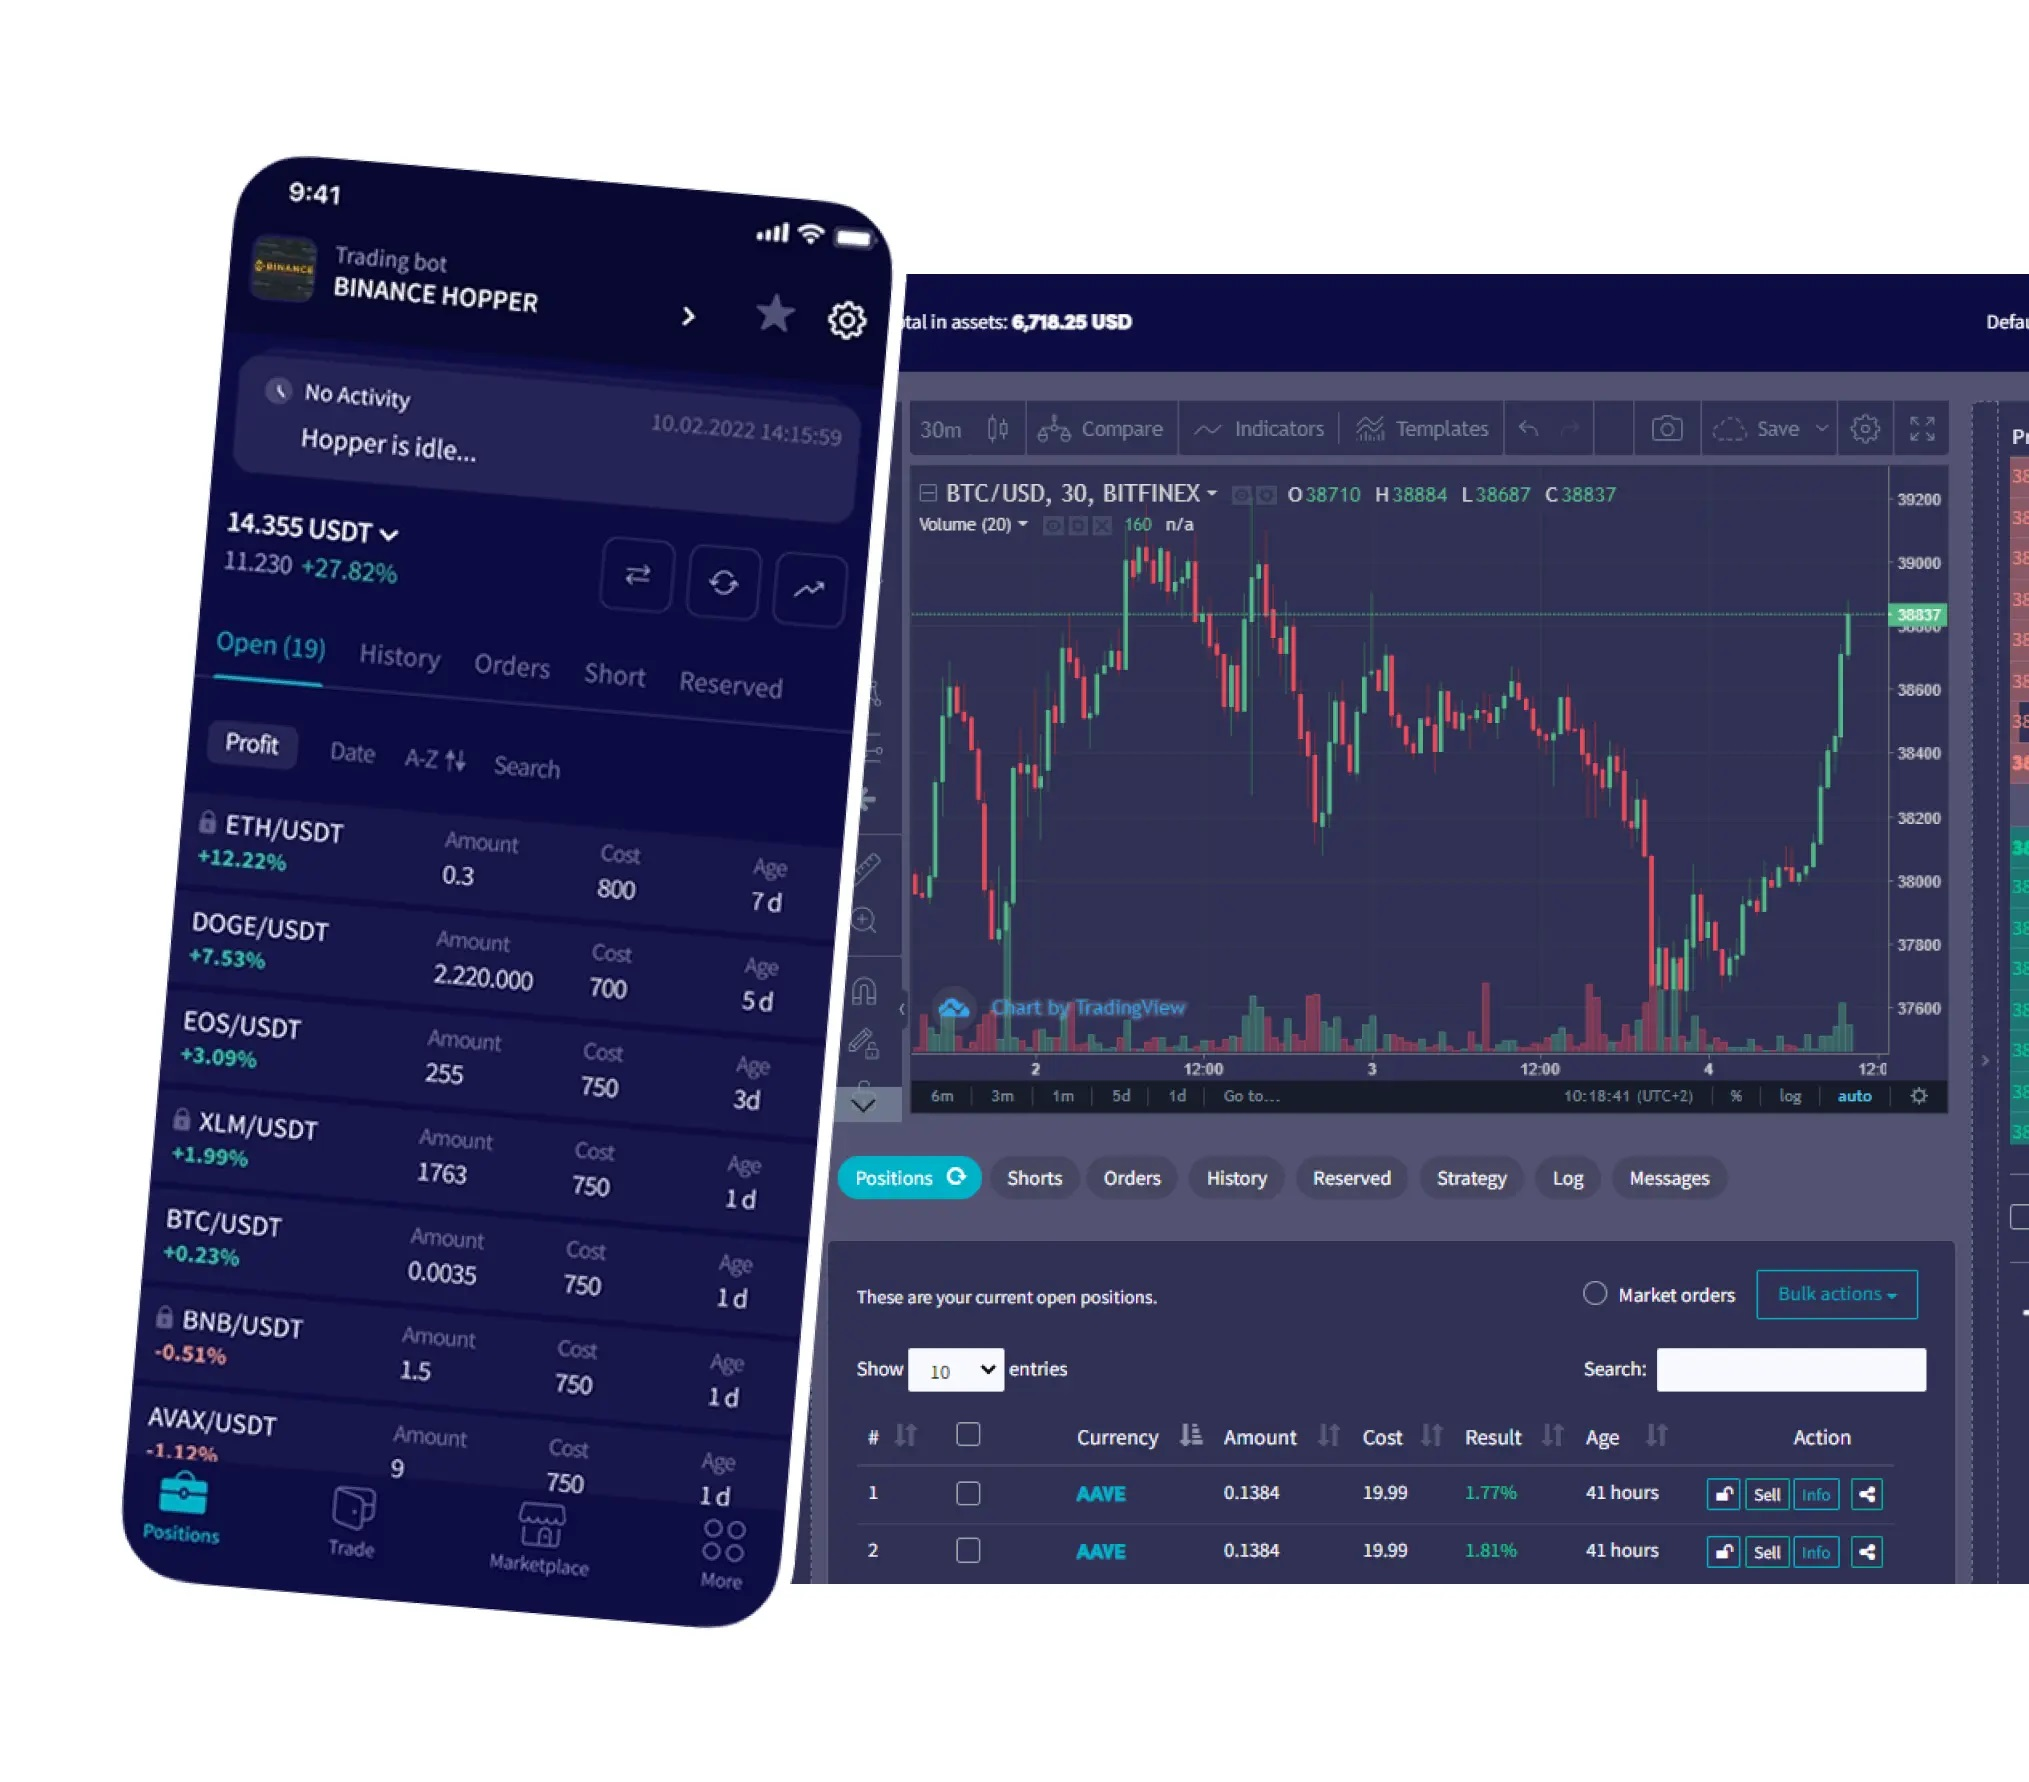
\includegraphics[scale=0.2]{trade}
	\centering
	\caption{ربات  معاملات خودکار برای  بازار ارز های دیجیتال}
	\cite{cryptohopper}
	\label{trade:fig1}
\end{figure} 
\section{طرح مسئله}
در
\cite{tran2023optimizing}
به سیستم های معامله گر خودکار برای بازار ارزهای دیجیتال بر اساس یادگیری تقویتی اشاره شده است . یک سیستم که بتواند بدون دخالت انسان و به صورت خودمختار با توجه به داده های بازار معاملاتی را انجام دهد و با استفاده از یادگیری تقویتی عمیق بیشترین سود را از معاملات بدست آورد .

\section{مدل\lr{PEAS}} 
سیستم های معامله گر خودکار به صورت سامانه هایی هوشمند می توانند تصمیمات مناسب را به دور از هیجاناتی که انسان ها دچار آن می شوند معاملات را طبق قوانین معلوم انجام دهند . در ادامه به بررسی مدل این سیستم ها می کنیم .
\subsection{اندازه گیری عمکرد} 
برای اندازه گیری عملکرد یک چنین سیستم هایی می توان به سود ماهیانه ی آن ها توجه کرد . در 
\cite{tran2023optimizing}
بهترین و بدترین و مقدار متوسط سود ماهیانه به عنوان تابع عملکرد و تابع جایزه یادگیری تقویتی در نظر گرفته شده اند .
\subsection{محیط}
محیط در مورد مسئله ی فوق مجموعه حالت هایی است که سیستم می تواند در آن ها قرار گیرد . حالت این سیستم می تواند با میزان دارایی ها و سرمایه ی سیستم به علاوه ی اطلاعات قیمت کالای معاملاتی - که در این جا ارز دیجیتال است - باشد . 
\par 
محیط به صورت کامل رویت پذیر
\footnote{\lr{fully observable}}
می باشد . محیط دائم در حال تغییر است و بنابراین به صورت پویا
\footnote{\lr{dynamic}}
است . این نکته مهم است که این تغییرات می توانند به صورت تصادفی باشند و گاهی قیمت کالایی نوسان داشته باشد . طبیعتا در بازار کاربران دیگری هم در حال معامله می باشند و محیط به صورت چند کاربره است . 
محیط به صورت 
\lr{episodic}
می باشد و به علت بزرگ بودن بازار رفتار محیط به 
\lr{action}
های 
\lr{agent} 
وابسته نیست . 
هم چنین تغییرات سیستم به صورت گسسته در نظرگرفته شده است .

\subsection{عملگر}
عملیات های سیتم باید توسط برخی از قوانین که برای نرم افزار تعریف شده اند محدود شوند . عملیات های نرم افزار متنوع هستند و می توانند شامل فروش مقداری خاص از نوعی ارز  باشند .
\subsection{حسگر}
به منظور تشخیص وضعیت بازار نیاز است سیستم مستقیم به سایت معاملاتی اتصال داشته باشد و اطلاعات مورد نیاز خود از محیط را به صورت سیگنال هایی از آن دریافت نماید .
\section{جمع بندی}
در فصل فعلی به بررسی کلی از سامانه  های معامله گر پرداختیم و به صورت کلی به شیوه ی عملکرد آن ها پرداختیم . هر یک از عملیات هایی که ربات معامله گر انجام می دهند با توجه به 
\lr{rationality}
است و سعی دارد تا پاسخ مناسب بدهند وتابع سود را بیشینه کند .






%
\chapter{پیشنهاد دهنده کالا وخدمات }
\section{مقدمه}

 در سال های اخیر خرید کالا ویا استفاده از خدمات آنلاین افزایش یافته است . 
سیستم‌های پیشنهاد ‌کننده ابزارهای مهمی برای مصرف کنندگان برای شناسایی کالاها وخدمات مورد علاقه خود و نیز برای کسب‌وکارها برای بهبود محصولات و خدمات خود هستند.
انتخاب و رزرو هتل 
 \cite{abbasi2019grouping}
یا رستوران
\cite{asani2021restaurant}
به صورت آنلاین هم شاهد رشد پررونقی بوده است و نقش این پیشنهاد دهنده های هوشمند در این رشد موثر بوده است ؛ در ادامه به بررسی یکی از این سیستم های پیشنهاد دهنده هتل به عنوان عامل هوشمند می پردازیم . 
\begin{figure}[h]
	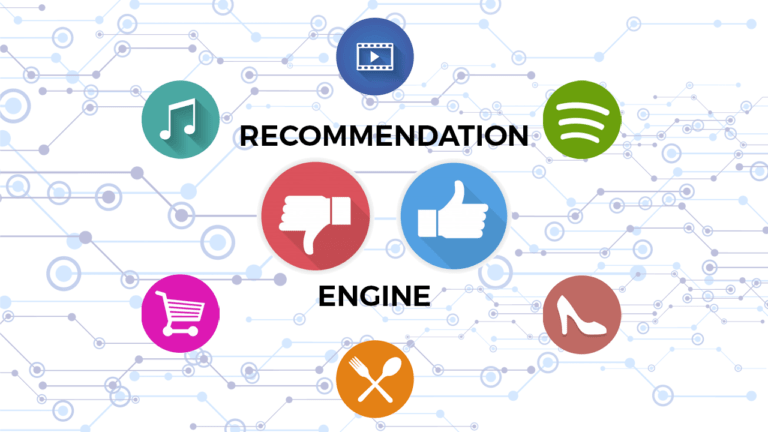
\includegraphics[scale=0.5]{reccomendation_sys}
	\centering
	\caption{موتورهای پیشنهاد دهنده کالا و خدمات}
	\cite{Naveennomidl}
	\label{rec_sys:fig1}
\end{figure} 
\section{طرح مسئله}
سیستم‌های توصیه‌کننده به عنوان یکی از عوامل موثر در رونق برخی از پلتفرم های آنلاین به شمار می روند . این سیستم ها براساس داده های رضایتمندی مشتریان ، میزان فروش کالا و خدمات وسلیقه و علاقه مندی افراد به ارائه پیشنهاد به منظور افزایش رضایت کاربران می پردازند . در 
 \cite{abbasi2019grouping}
 با هدف طراحی یک سیستم توصیه‌کننده بر اساس ترجیحات صریح و ضمنی مشتریان پرداخته شده است . این توصیه کننده برای پیشنهاد هتل طراحی شده است .
\section{مدل\lr{PEAS}} 
در این بخش به بررسی هوشمندی این سیستم توصیه کننده می پردازیم ؛ این سیستم را از نظر ویژگی های عملکرد ،  محیط ، عملگرها و حسگرها می سنجیم .
\subsection{اندازه گیری عمکرد} 
عملکرد چنین سیستمی را  می توان با امتیازات کاربران به پیشنهاد سیستم سنجید . همچنین تعداد مشتریان هم می تواند معیار مفیدی در دراز مدت باشد .
\subsection{محیط}
محیط در این مسئله را می توان به مجموعه ی تمام هتل ها و اتاق های آن ها تعبیر نمود .
محیط به صورت کامل رویت پذیر
است و نیز با توجه به این که قیمت و کیفیت خدمات هتل ها وشرایط گردشگری و مسافرتی کشور ها می توانند به مرور تغییر کنند و بنابراین محیط  به صورت پویا است . این نکته مهم است که این تغییرات می توانند به صورت تصادفی باشند و در نتیجه محیط تصادفی است . محیط را می توان به صورت تک کاربره در نظر گرفت (اثرات بقیه پیشنهاد کننده ها را می توان نادیده گرفت). 
هم چنین تغییرات سیستم را  به صورت گسسته می توان در نظر گرفت .


\subsection{عملگر}
عملیات های سیستم به این صورت می باشند که یک با توجه به شرایط اتاق های هتل ها به کاربر پیشنهاد دهند و همین پیشنهاد دادن ها عملیات های سیستم تلقی می شوند .
\subsection{حسگر}
سیستم از طریق امتیازات و رضایتمندی کاربران و قیمت هایی که هتل ها اعلام می کنند می تواند به علاقه مشتریان و کیفیت هتل ها پی ببرد ؛ این موارد به عنوان باز خورد ازمحیط شمرده شوند .
\section{جمع بندی}
درانتها این نکته را ذکر می می کنیم که هر یک از پیشنهاد هایی که یک سیستم پیشنهاد کننده ارائه می کند با توجه به 
\lr{rationality}
است و بر مبنای شناختی که از مخاطب دارد می باشد ودر نتیجه  پاسخ مناسب تری دریافت شود و تابع مطلوبیت یعنی فروش و رضایتمندی مشتری است ؛ بیشینه شود .


%\chapter{جمع بندی و نتیجه گیری}
با پیشرفت فناوری های جدید ، ساخت وسایل هوشمند را به همراه داشته است . الگوریتم های یادگیری ماشین شامل یادگیری تقویتی و شبکه های عصبی و همین طور الگوریتم های مربوط به بینایی ماشین در پیشبرد هوشمند سازی وسایل ساخته ی بشر نقش اساسی داشته اند . این عامل های هوشمند هر یک می توانند در مسائل مختلف بر اساس نوعی عقلانیت تصمیم گیری کنند و بدون نیاز به نوشتن الگوریتم های متعدد کار ها و عملیات های متفاوتی را انجام دهند . در این گزارش سعی شد تا به تنوع این عوامل هوش مصنوعی و ویژگی های هریک و محیط هایی که در آن عمل می کنند ، پرداخته  شود .  
%--------------------------------------------------------------------------appendix( مراجع و پیوست ها)
\chapterfont{\vspace*{-2em}\centering\LARGE}%
\appendix
\bibliographystyle{plain-fa}

\bibliography{references}

%\chapter*{‌پیوست}
\markboth{پیوست}{}
\addcontentsline{toc}{chapter}{پیوست}
موضوعات مرتبط با متن گزارش پایان نامه كه در يكی از گروه‌های زير قرار می‌گيرد، در بخش پيوست‌ها آورده شوند:
\begin{enumerate}
\item  اثبات های رياضی يا عمليات رياضی طولانی‌.‌
\item داده و اطلاعات نمونه (های) مورد مطالعه (\lr{Case Study}) چنانچه طولانی باشد‌.‌
\item نتايج كارهای ديگران چنانچه نياز به تفصيل باشد‌.‌
\item مجموعه تعاريف متغيرها و پارامترها، چنانچه طولانی بوده و در متن به انجام نرسيده باشد‌.‌
\end{enumerate}
% براي شماره‌گذاري روابط، جداول و اشكال موجود در پيوست‌ از ساختار متفاوتي نسبت به متن اصلي استفاده مي‌شود كه در زير به‌عنوان نمونه نمايش داده شده‌است. 
% \begin{equation}
%F=ma
%\end{equation}
\section*{کد میپل }
\begin{latin}
\begin{verbatim}

with(DifferentialGeometry):
with(Tensor):
DGsetup([x, y, z], M)
																	frame name: M
a := evalDG(D_x)
																	D_x
b := evalDG(-2 y z D_x+2 x D_y/z^3-D_z/z^2)


\end{verbatim}
\end{latin}
%--------------------------------------------------------------------------dictionary(واژه نامه ها)s
%اگر مایل به داشتن صفحه واژه‌نامه نیستید، خط زیر را غیر فعال کنید.
%\parindent=0pt
%%
\chapter*{واژه‌نامه‌ی فارسی به انگلیسی}
\pagestyle{style9}

\addcontentsline{toc}{chapter}{واژه‌نامه‌ی فارسی به انگلیسی}
%%%%%%
\begin{multicols*}{2}

{\bf آ}
\vspace*{3mm}


\farsiTOenglish{اسکالر}{Scalar}


\vspace*{3mm}
{\bf ب}
\vspace*{3mm}

\farsiTOenglish{بالابر}{Lift}


\vspace*{3mm}
{\bf پ}
%%\vspace*{3mm}

\farsiTOenglish{پایا}{Invariant}



\vspace*{3mm}
{\bf ت}
%%\vspace*{3mm}

\farsiTOenglish{ تناظر }{Correspondence}


\vspace*{3mm}
{\bf ث}
%%\vspace*{3mm}

\farsiTOenglish{ثابت‌ساز}{Stabilizer}

\vspace*{3mm}
{\bf ج}
%%\vspace*{3mm}

\farsiTOenglish{جایگشت}{Permutation}



\vspace*{3mm}
{\bf چ}
%%\vspace*{3mm}


\farsiTOenglish{چند جمله‌ای }{Polynomial}

\vspace*{3mm}
{\bf ح}
%%\vspace*{3mm}

\farsiTOenglish{حاصل‌ضرب دکارتی}{Cartesian product}


\vspace*{3mm}
{\bf خ}
%%\vspace*{3mm}

\farsiTOenglish{خودریختی}{Automorphism}

\vspace*{3mm}
{\bf د}
%%\vspace*{3mm}

\farsiTOenglish{درجه}{Degree}


\vspace*{3mm}
{\bf ر}
%%\vspace*{3mm}


\farsiTOenglish{ریزپردازنده}{microprocessor}


\vspace*{3mm}
{\bf ز}
%%\vspace*{3mm}


\farsiTOenglish{زیرمدول}{Submodule}


\vspace*{3mm}
{\bf س}
%%\vspace*{3mm}

\farsiTOenglish{سرشت}{Character}


\vspace*{3mm}
{\bf ص}
%%\vspace*{3mm}

\farsiTOenglish{صادقانه}{Faithful}

\vspace*{3mm}
{\bf ض}
%%\vspace*{3mm}

\farsiTOenglish{ضرب داخلی}{Inner product}

\vspace*{3mm}
{\bf ط}
%%\vspace*{3mm}


\farsiTOenglish{طوقه}{Loop}


\vspace*{3mm}
{\bf ظ}
%%\vspace*{3mm}


\farsiTOenglish{ظرفیت}{Valency}
 
\vspace*{3mm}
{\bf ع}
%%\vspace*{3mm}


\farsiTOenglish{عدم مجاورت}{Nonadjacency}



\vspace*{3mm}
{\bf ف}
%%\vspace*{3mm}

\farsiTOenglish{فضای برداری}{Vector space}



\vspace*{3mm}
{\bf ک}
%%\vspace*{3mm}

\farsiTOenglish{کاملاً تحویل‌پذیر}{Complete reducibility}


\vspace*{3mm}
{\bf گ}
%%\vspace*{3mm}


\farsiTOenglish{گراف}{Graph}



\vspace*{3mm}
{\bf م}
%%\vspace*{3mm}

\farsiTOenglish{ماتریس جایگشتی}{Permutation matrix }


\vspace*{3mm}
{\bf ن}
%%\vspace*{3mm}

\farsiTOenglish{ناهمبند}{Disconnected}


\vspace*{3mm}
{\bf و}
%%\vspace*{3mm}

\farsiTOenglish{وارون‌پذیر}{Invertible}


\vspace*{3mm}
{\bf ه}
%%\vspace*{3mm}

\farsiTOenglish{همبند}{Connected}



\vspace*{3mm}
{\bf ی}
%%\vspace*{3mm}

\farsiTOenglish{یال}{Edge}




\end{multicols*}%
%%%%%%%
\chapter*{ واژه‌نامه‌ی انگلیسی به فارسی}
\pagestyle{style9}
\lhead{\thepage}\rhead{واژه‌نامه‌ی انگلیسی به فارسی}
\addcontentsline{toc}{chapter}{واژه‌نامه‌ی انگلیسی به فارسی}

\LTRmulticolcolumns
\begin{multicols}{2}
{\hfill\bf  \lr{A}}
%%\vspace*{1.5mm}

\englishTOfarsi{Automorphism}{خودریختی}

\vspace*{3mm}
{\hfill\bf   \lr{B}}
%%\vspace*{1.5mm}

\englishTOfarsi{Bijection}{دوسویی}

\vspace*{3mm}
{\hfill\bf   \lr{C}}
%%\vspace*{1.5mm}

\englishTOfarsi{Cycle group}{گروه دوری}

\vspace*{3mm}
{\hfill\bf   \lr{D}}
%%\vspace*{1.5mm}

\englishTOfarsi{Degree}{درجه}

\vspace*{3mm}
{\hfill\bf   \lr{E}}
%%\vspace*{1.5mm}

\englishTOfarsi{Edge}{یال}

\vspace*{3mm}
{\hfill\bf   \lr{F}}
%%\vspace*{1.5mm}

\englishTOfarsi{Function}{تابع}

\vspace*{3mm}
{\hfill\bf   \lr{G}}
%%\vspace*{1.5mm}

\englishTOfarsi{Group}{گروه}

\vspace*{3mm}
{\hfill\bf   \lr{H}}
%%\vspace*{1.5mm}

\englishTOfarsi{Homomorphism}{همریختی}

\vspace*{3mm}
{\hfill\bf   \lr{I}}
%%\vspace*{1.5mm}

\englishTOfarsi{Invariant}{پایا}

\vspace*{3mm}
{\hfill\bf   \lr{L}}
%%\vspace*{1.5mm}

\englishTOfarsi{Lift}{بالابر}

\vspace*{3mm}
{\hfill\bf   \lr{M}}
%%\vspace*{1.5mm}

\englishTOfarsi{Module}{مدول}

\vspace*{3mm}
{\hfill\bf   \lr{N}}
%%\vspace*{1.5mm}

\englishTOfarsi{Natural map}{نگاشت طبیعی}

\vspace*{3mm}
{\hfill\bf   \lr{O}}
%%\vspace*{1.5mm}

\englishTOfarsi{One to One}{یک به یک}

\vspace*{3mm}
{\hfill\bf   \lr{P}}
%%\vspace*{1.5mm}

\englishTOfarsi{Permutation group}{گروه جایگشتی}

\vspace*{3mm}
{\hfill\bf   \lr{Q}}
%%\vspace*{1.5mm}

\englishTOfarsi{Quotient graph}{گراف خارج‌قسمتی}

 \vspace*{3mm}
{\hfill\bf   \lr{R}}
%%\vspace*{1.5mm}

\englishTOfarsi{Reducible}{تحویل پذیر}

\vspace*{3mm}
{\hfill\bf   \lr{S}}
%%\vspace*{1.5mm}

\englishTOfarsi{Sequence}{دنباله}

 \vspace*{3mm}
{\hfill\bf   \lr{T}}
%%\vspace*{1.5mm}

\englishTOfarsi{Trivial character}{سرشت بدیهی}

\vspace*{3mm}
{\hfill\bf   \lr{U}}
%%\vspace*{1.5mm}

\englishTOfarsi{Unique}{منحصربفرد}

\vspace*{3mm}
{\hfill\bf   \lr{V}}
%%\vspace*{1.5mm}

\englishTOfarsi{Vector space}{فضای برداری}
\end{multicols}
%--------------------------------------------------------------------------index(نمایه)
%اگر مایل به داشتن صفحه نمایه نیستید، خط زیر را غیر فعال کنید.
%\pagestyle{style7}
%\printindex
%\pagestyle{style7}

%%کلمات کلیدی انگلیسی
\latinkeywords{Write a 3 to 5 KeyWords is essential. Example: AUT, M.Sc., Ph. D,..}
%چکیده انگلیسی

\en-abstract{
This page is accurate translation from Persian abstract into English.
}
%%%%%%%%%%%%%%%%%%%%% کدهای زیر را تغییر ندهید.

\newpage
\thispagestyle{empty}
\begin{latin}
\section*{\LARGE\centering Abstract}

\een-abstract

\vspace*{.5cm}
{\large\textbf{Key Words:}}\par
\vspace*{.5cm}
\elatinkeywords
\end{latin}
%% در این فایل، عنوان پایان‌نامه، مشخصات خود و چکیده پایان‌نامه را به انگلیسی، وارد کنید.
%%%%%%%%%%%%%%%%%%%%%%%%%%%%%%%%%%%%
\baselineskip=.6cm
\begin{latin}

\latinfaculty{Department of ...}


\latintitle{Title of Thesis}


\firstlatinsupervisor{Dr. }

%\secondlatinsupervisor{Second Supervisor}

\firstlatinadvisor{Dr. }

%\secondlatinadvisor{Second Advisor}

\latinname{Name}

\latinsurname{Surname}

\latinthesisdate{Month \& Year}

\latinvtitle
\end{latin}


\end{document}